% Final-project report: When Does LLM-Driven Memory Construction Help?
% ACL format (acl.sty)

\documentclass[11pt]{article}

% Final / camera-ready (non-anonymous). Switch to [review] for double-blind.
\usepackage{acl}

% Standard packages required by the official ACL template.
\usepackage{times}
\usepackage{latexsym}
\usepackage[T1]{fontenc}
\usepackage[utf8]{inputenc}
\usepackage{microtype}
\usepackage{inconsolata}

% Project-specific packages (figures, tables, math).
\usepackage{graphicx}
\usepackage{booktabs}
\usepackage{amsmath}
\usepackage{amssymb}
\usepackage{multirow}
\usepackage{array}
\usepackage{url}

\title{When Does {LLM}-Driven Memory Construction Help?\\
A Controlled Empirical Study on Long-Term Conversational QA}

\author{Yong Yang \\
  School of Software \\
  Beihang University \\
  \texttt{yang\_qhd@buaa.edu.cn}}

\begin{document}
\maketitle

\begin{abstract}
Recent long-term-memory systems for LLM agents, including
Mem0~\citep{chhikara2025mem0}, Zep~\citep{rasmussen2025zep} and
MemOS~\citep{li2025memos}, all share a common assumption: that asking
an LLM to extract, summarise or otherwise rewrite the raw conversation
into structured memory items is worth its construction cost. We
question that assumption with a controlled study on
LongMemEval-S~\citep{wu2024longmemeval}, in which we hold the encoder
(BGE-M3), the cross-encoder reranker (\texttt{bge-reranker-base}) and
the generator (Qwen2.5-7B-Instruct) fixed, match every retriever to a
1024-token context budget, and vary only the construction pipeline.
On the shared 50-question subset, a plain Dense + reranker retriever
reaches 54\% accuracy, statistically indistinguishable from an Oracle
upper bound of 56\% (paired McNemar $p=1.0$). Substituting the same
chunks with LLM-generated session summaries
(``Dense-Summarised'') drops accuracy to 34\%, and a Mem0-style
add/update/delete/no-op extractor on the 7B model collapses to 8\%.
Diagnostic analysis attributes both regressions to the same root
cause: lossy paraphrasing during construction strips out the
literal numbers, dates and entity strings that the encoder relies on
to match a question. The take-away for practitioners is that under a
small open-weight generator, a strong off-the-shelf retriever already
saturates the retrieval bottleneck, and adding an LLM construction
stage is more likely to hurt than to help.
\end{abstract}

%================================================
\section{Introduction}
\label{sec:intro}

A persistent LLM agent has to remember information across context
resets~\citep{liu2023lost}, and the dominant solution is to
externalise memory along three canonical axes
\citep{li2025memos,chhikara2025mem0,rasmussen2025zep}: construction,
storage and retrieval. Our companion survey~\citep{yang2026survey}
reviews each axis with one representative 2025 system. The present
project is the empirical counterpart of that survey, focused on the
construction axis.

Most published evidence in favour of LLM-driven construction comes
from headline numbers reported on top of large proprietary
generators (GPT-4o, GPT-4-turbo). Whether those gains transfer to a
single-A800 deployment with a 7B-class open-weight generator is, in
our reading, an open question, and one that practitioners on a
budget actually care about. We therefore design a study that holds
everything except the construction pipeline fixed.

\noindent\textbf{Research questions.}
\begin{itemize}
  \setlength{\itemsep}{2pt}
  \setlength{\topsep}{2pt}
  \item \textbf{RQ1.} At a matched 1024-token context budget, does
        LLM-driven memory construction outperform a plain
        Dense + reranker retriever on long-conversation QA?
  \item \textbf{RQ2.} If a gap exists in either direction, can it be
        attributed to memory \emph{granularity}
        (passage chunks vs.\ sentence-level facts), or to the
        four-operation update agent that resolves contradictions?
  \item \textbf{RQ3.} What latency and token-cost penalties does the
        construction stage actually incur, relative to the accuracy it
        delivers?
\end{itemize}

\noindent\textbf{Contributions.}
(i) An open-source benchmark stack with seven retrievers
(\textsc{One-hot}, \textsc{TF-IDF}, BM25, Dense+Reranker,
Dense-Summarised, Mem0-Lite, Oracle) sharing one entry point,
one prompt template, one judge and one token budget; (ii) a
matched comparison on the shared 50-question subset of
LongMemEval-S with paired McNemar tests and bootstrap 95\% CIs;
(iii) a diagnostic analysis that traces two unexpected regressions
(Dense-Summarised and Mem0-Lite) back to a single mechanism rather
than to a long list of independent failures.

%================================================
\section{Related Work}
\label{sec:related}

We refer the reader to our survey~\citep{yang2026survey} for a fuller
treatment. Briefly, classical IR
(BM25~\citep{robertson2009bm25}) and dense
retrieval~\citep{karpukhin2020dpr} are the workhorses of
RAG~\citep{lewis2020rag}; both perform passage-level lookup over the
raw conversation. \textbf{Mem0}~\citep{chhikara2025mem0} replaces
passages with LLM-extracted memory items managed via
\textsc{Add}/\textsc{Update}/\textsc{Delete}/\textsc{Noop}; this is
the construction pattern we replicate as Mem0-Lite.
\textbf{Zep}~\citep{rasmussen2025zep} layers a temporally-aware
knowledge graph on top of storage and retrieval, and
\textbf{MemOS}~\citep{li2025memos} treats memory as a first-class
operating-system resource. The latter two are out of scope for the
construction-axis study reported here. The closest published
ablation we are aware of is the cost-vs-accuracy analysis in the
Mem0 paper itself~\citep{chhikara2025mem0}, which compares Mem0
against a 128K full-context baseline; our setup is different in
that we ablate the construction stage \emph{within} a fixed-budget
RAG pipeline rather than against full context.

%================================================
\section{Models}
\label{sec:methods}

All systems share the same I/O contract: given a multi-session
conversation $\mathcal{H}$ and a question $q$, return an answer
$\hat{a}$. They differ only in how they obtain a memory context
$\beta$, which is then concatenated with $q$ in a fixed prompt
template (Appendix). All retrievers are packed to the same
\textbf{token budget} $B{=}1024$ before generation, so that
differences trace back to memory \emph{quality} rather than
\emph{quantity}.

\paragraph{(I) Classical IR baselines.}
\textsc{One-hot} uses binary term-presence bag-of-words
(scikit-learn \texttt{CountVectorizer}, \texttt{binary=True}) scored
by cosine; \textsc{TF-IDF} uses sublinear bigram TF-IDF with L2
normalisation (cosine via inner product); \textsc{BM25} uses the
Okapi formulation from \texttt{rank\_bm25} with default parameters.
Sessions are concatenated and split into 512-character chunks. We
include the One-hot $\to$ $n$-gram TF-IDF $\to$ BM25 ladder so that
the neural systems can be calibrated against the classical IR
results that motivated the field.

\paragraph{(II) Dense + reranker.}
The same chunks are encoded with \textbf{BGE-M3}~\citep{chen2024bgem3}
(unit-norm sentence embeddings via \texttt{sentence\_transformers})
and shortlisted by inner product against the query embedding; a
\textbf{cross-encoder} reranker (\texttt{BAAI/bge-reranker-base})
re-orders the top-32 shortlist before truncation to top-$k$. This is
our strongest off-the-shelf dense baseline, and the one against which
the construction-side variants are most directly compared.

\paragraph{(III) Dense-Summarised.}
A critical isolation baseline. Each session is summarised by the
generator LLM into a short JSON list of third-person facts, capped
at 12 facts per session; those facts are then dense-indexed and
retrieved with \emph{the same} cross-encoder reranker as in (II).
Dense vs.\ Dense-Summarised therefore isolates the effect of
\emph{granularity / construction} (passage vs.\ LLM-rewritten fact)
from that of the rerank stage and the encoder, both of which are now
shared.

\paragraph{(IV) Mem0-Lite.}
Faithfully follows Mem0's two-phase pipeline: (a)~per
\texttt{(user, assistant)} pair, an LLM \emph{extractor} emits typed
memory items as JSON (episodic / semantic / user-profile); (b)~each
candidate is compared against the top-5 most similar memories
already in the bank, and an LLM \emph{updater} commits one of
\textsc{Add}/\textsc{Update}/\textsc{Delete}/\textsc{Noop}. We use
the same Qwen2.5-7B-Instruct as both extractor and updater so that
all variation is in the construction logic, not in model strength.

\paragraph{(V) Oracle.}
Reads LongMemEval's gold \texttt{has\_answer} flag on each turn and
returns those turns as memories. This provides a retrieval-perfect
upper bound; the gap between Oracle and any other retriever is the
remaining headroom for retrieval improvements at the same generator.

%================================================
\section{Evaluation}
\label{sec:setup}

\paragraph{Data.}
LongMemEval-S~\citep{wu2024longmemeval}: $\sim$115K-token haystacks
across six question types (single-session-user,
single-session-assistant, single-session-preference, multi-session,
temporal-reasoning, knowledge-update). We use \emph{prefix-stable}
subsampling: the dataset is shuffled once with seed 42, and the
first $N$ questions are taken. The cheap retrievers
(\textsc{One-hot}, \textsc{TF-IDF}, BM25, Dense, Dense-Summarised,
Oracle) are evaluated on $N{=}200$; the construction-heavy Mem0-Lite
run uses $N{=}50$ because its indexing is $O(\text{turns})$ with two
LLM calls per turn. Because of prefix-stability, the $N{=}50$
subset is a strict prefix of the $N{=}200$ subset, so the
cross-system comparison on the shared 50-question subset is
well-defined; this is the comparison we report as the primary
result.

\paragraph{Models.}
\textbf{Generator}: Qwen2.5-7B-Instruct (bf16, A800 80G, HuggingFace
Transformers backend, SDPA attention, greedy decoding).
\textbf{Encoder}: BGE-M3. \textbf{Reranker}:
\texttt{bge-reranker-base}, applied to both Dense and
Dense-Summarised so that the rerank stage is no longer a confounder.
\textbf{Judge}: a different model family from the generator,
DeepSeek-V4-Flash via its OpenAI-compatible API, to mitigate
self-preference bias~\citep{panickssery2024selfpref}.

\paragraph{Metrics.}
(i) \textbf{Accuracy} from a strict-JSON LLM-as-judge
prompt (Appendix); on the shared 50-question subset we additionally
report (ii) bootstrap 95\% CIs (10\,000 resamples) and (iii) paired
\textbf{McNemar} tests across all system pairs, computed without a
SciPy dependency: the discordant-pair count is small ($<25$) for
every comparison so we use the exact two-sided binomial tail. We
also log \textbf{p50/p95 indexing latency},
\textbf{p50/p95 generation latency} (with
\texttt{torch.cuda.synchronize()} and a one-question warm-up), and
both prompt and completion tokens.

\paragraph{Reproducibility.}
All LLM calls are content-addressed and disk-cached, so a re-run on
the same machine reproduces the numbers bit-for-bit. We additionally
seed Python, NumPy and PyTorch, drop the first-sample timing as a
warm-up, and ship the full configuration as YAML files under
\texttt{configs/}. A single command,
\texttt{bash scripts/run\_all.sh}, reproduces the seven runs end to
end; \texttt{python -m src.aggregate} produces the summary CSV and
\texttt{python -m src.plot\_results} produces every figure in this
paper.

%================================================
\section{Results}
\label{sec:results}

We first report the headline accuracy and significance results
(Table~\ref{tab:results}, Fig.~\ref{fig:bar}), then walk through the
three contrasts that motivate the study, and finally diagnose the
two unexpected regressions.

\begin{table}[t]
\centering
\footnotesize
\setlength{\tabcolsep}{4pt}
\renewcommand{\arraystretch}{1.15}
\begin{tabular}{@{}l c c r r@{}}
\toprule
\textbf{Retriever} & \textbf{Acc.} & \textbf{95\% CI} & \textbf{Idx (s)} & \textbf{Tok\,in} \\
\midrule
One-hot              & 0.38          & {\scriptsize[0.24, 0.52]} &   0.06 & 220k   \\
TF-IDF               & 0.44          & {\scriptsize[0.30, 0.58]} &   0.16 & 228k   \\
BM25                 & 0.44          & {\scriptsize[0.30, 0.58]} &   0.06 & 230k   \\
Dense+rerank         & \textbf{0.54} & {\scriptsize[0.40, 0.68]} &   7.40 & 235k   \\
Dense-Summarised     & 0.34          & {\scriptsize[0.22, 0.48]} &  72.6  & 23.0M  \\
Mem0-Lite (7B)       & 0.08          & {\scriptsize[0.02, 0.16]} & 251.9  & 21.6M  \\
\midrule
Oracle (bound)       & 0.56          & {\scriptsize[0.42, 0.70]} &   0.00 & 104k   \\
\bottomrule
\end{tabular}
\caption{Accuracy on the shared 50-question subset of LongMemEval-S
at a matched 1024-token context budget, with bootstrap 95\%
confidence intervals. ``Idx'' is the median per-question
indexing/retrieval latency; ``Tok\,in'' is the cumulative number of
generator-input tokens across the run, including any tokens consumed
by the construction stage.}
\label{tab:results}
\end{table}

\begin{figure*}[t!]
\centering
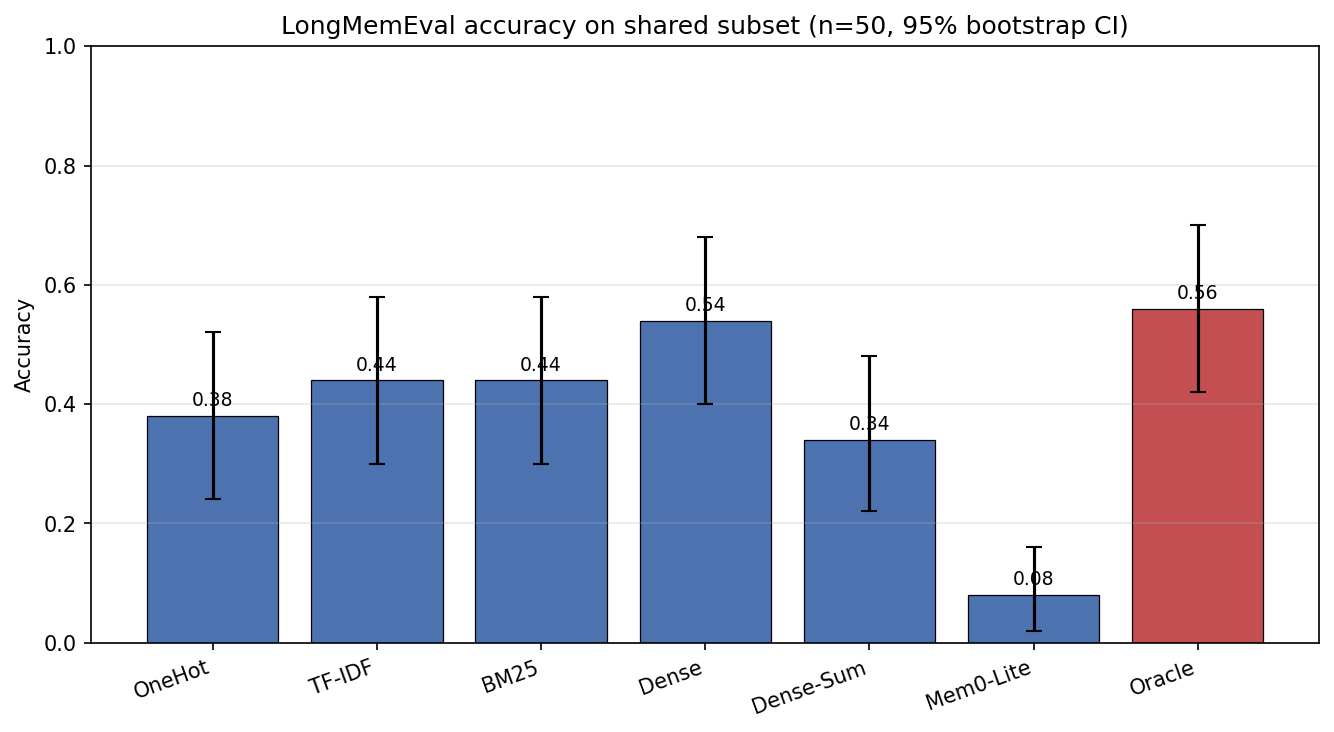
\includegraphics[width=0.85\textwidth]{figs/accuracy_bar.png}
\caption{Accuracy on the shared 50-question subset of LongMemEval-S
with 95\% bootstrap CIs. The Oracle bar is highlighted in red as
the retrieval-perfect upper bound; Dense lies within its CI.}
\label{fig:bar}
\end{figure*}

\paragraph{(a) Classical IR ladder.}
Moving from binary one-hot to bigram TF-IDF and BM25 lifts shared-50
accuracy from 0.38 to 0.44. Neither step is individually significant
(McNemar $p>0.4$), and TF-IDF and BM25 are tied within rounding,
which is what we would expect on conversational text where lexical
overlap already does most of the work. The classical ladder is
included as a sanity check: it calibrates the harder neural systems
against a familiar baseline and confirms that the pipeline is wired
correctly.

\paragraph{(b) Retrieval method (RQ1).}
Replacing BM25 with Dense + reranker lifts accuracy from 0.44 to
0.54; the McNemar comparison is borderline at $p=0.077$ on $n=50$ but
the discordant-pair pattern (8 cases where Dense is right and BM25
is wrong, against 3 in the other direction) is monotone in the
expected direction. More importantly, Dense at 0.54 is statistically
indistinguishable from the Oracle upper bound at 0.56 (paired
McNemar $p=1.0$, with 8 vs.\ 9 discordant pairs). Within the
1024-token budget, a vanilla BGE-M3 + cross-encoder pipeline is
already saturating the retrieval channel: any further accuracy gain
on this benchmark, with this generator, has to come from the
generator side rather than from a smarter retriever.

\paragraph{(c) Granularity / construction (RQ2).}
The Dense vs.\ Dense-Summarised contrast is the cleanest slice of
the experimental matrix, because both share an identical encoder,
shortlist size and cross-encoder reranker; the only difference is
that Dense-Summarised indexes LLM-generated facts instead of raw
chunks. Accuracy drops from 0.54 to 0.34, a 20-point gap with 17
``Dense correct, Dense-Summarised wrong'' pairs against 7 in the
other direction (McNemar $p=0.064$, on the borderline of
significance at $n=50$). At the same time, Dense-Summarised is
significantly worse than the Oracle bound ($p=0.019$). LLM
summarisation, instead of producing cleaner memory items, is
\emph{deleting} the very tokens that BGE-M3 needs to match the query
(see the diagnosis in \S\ref{sec:diagnosis}).

\paragraph{(d) Update agent (RQ2 cont.).}
Mem0-Lite, which adds the four-operation update agent on top of
LLM-extracted memory items, achieves only 0.08 accuracy on the
shared 50 questions. Every pairwise comparison with another system
is significant at $p<0.001$. Compared to the One-hot baseline, the
discordant-pair count is 0 in favour of Mem0-Lite against 15 in
favour of One-hot, that is, Mem0-Lite never recovers a question that
One-hot misses. On a 7B open-weight extractor / updater the update
agent does not realise the gains reported in the original Mem0
paper~\citep{chhikara2025mem0}; we discuss the failure mode in
\S\ref{sec:diagnosis}.

\paragraph{Cost / latency (RQ3).}
The cost ranking (Fig.~\ref{fig:cost}) is the inverse of the
accuracy ranking. One-hot, TF-IDF, BM25, Dense and Oracle all index
in well under one second per question and consume on the order of
$10^5$ generator-input tokens across the entire run. Dense-Summarised
spends 72.6\,s per question on indexing (one LLM call per session
for the summary) and ends up consuming roughly $2.3{\times}10^7$
input tokens, two orders of magnitude more than Dense at 20 points
lower accuracy. Mem0-Lite spends 252\,s per question on
construction (two LLM calls per turn) and a similar token volume,
while reaching the lowest accuracy of the seven systems. All of the
construction-heavy variants therefore sit in the bottom-right
quadrant of the accuracy-vs-cost plot: more expensive \emph{and}
less accurate.

\begin{figure*}[t!]
\centering
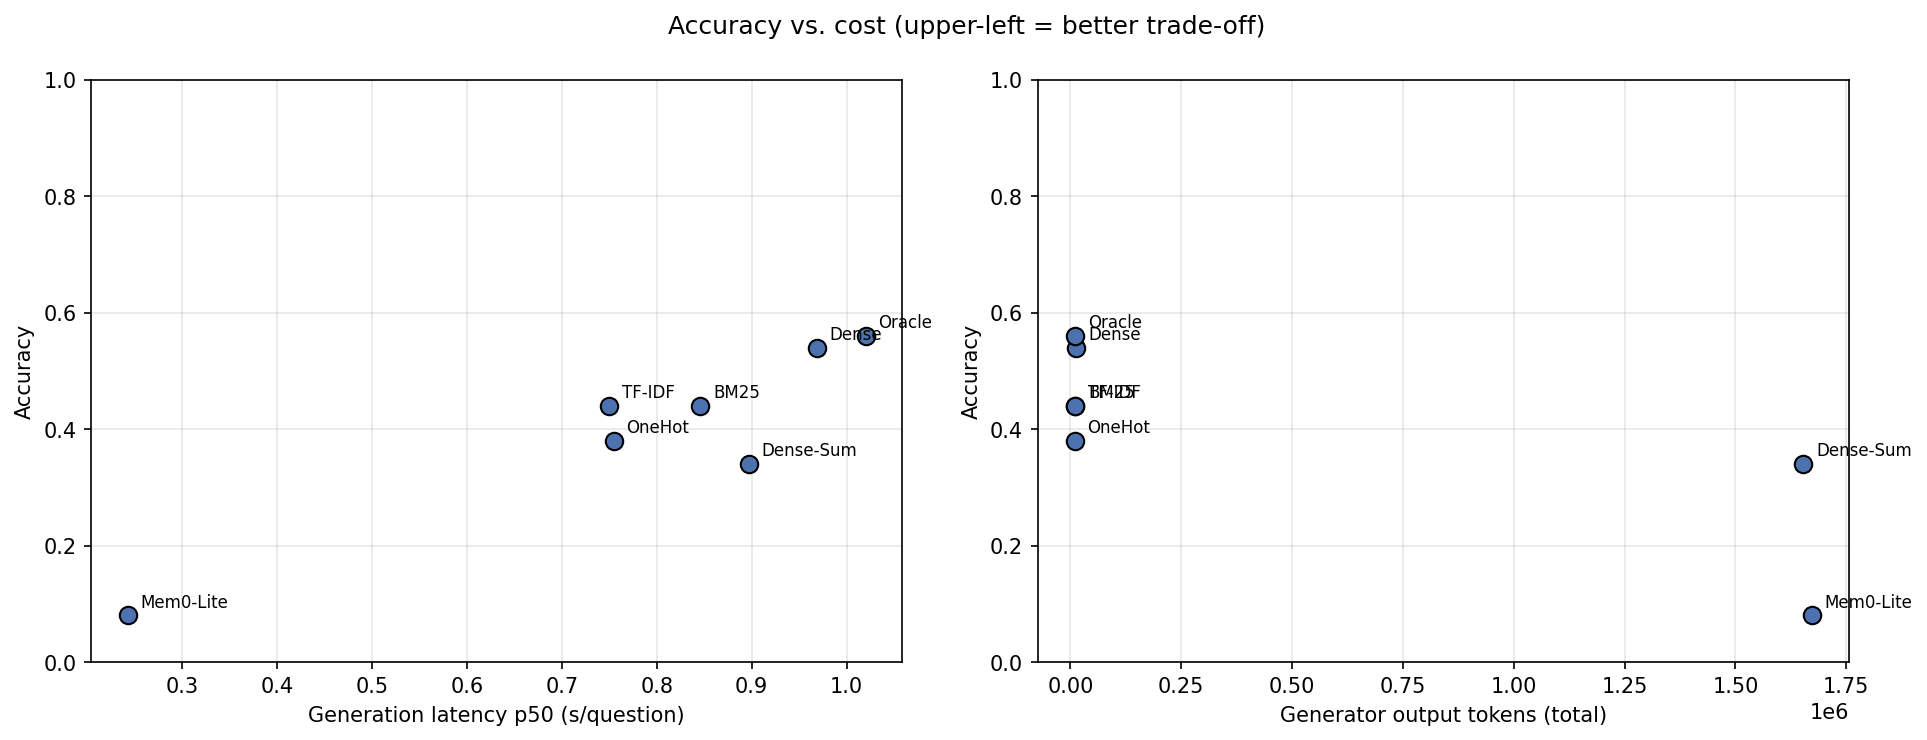
\includegraphics[width=0.92\textwidth]{figs/acc_vs_cost.png}
\caption{Accuracy vs.\ cost. Left: median per-question indexing
latency. Right: cumulative generator-input tokens. Upper-left is the
Pareto-preferred corner; the construction-heavy variants
(Dense-Summarised, Mem0-Lite) are far from it.}
\label{fig:cost}
\end{figure*}

\paragraph{Per-question-type breakdown.}
Fig.~\ref{fig:heat} shows accuracy stratified by the six
LongMemEval-S question types. Because each type has fewer than ten
questions on the shared subset, this view is qualitative only and
should not be used to claim significance per type. Single-session-user
is the easiest type for every retriever and the one on which Dense
reaches Oracle parity; multi-session and temporal-reasoning are the
hardest, and they are also where Mem0-Lite degrades most relative to
the other systems. This pattern is consistent with the
literal-information-loss diagnosis below.

\begin{figure*}[t!]
\centering
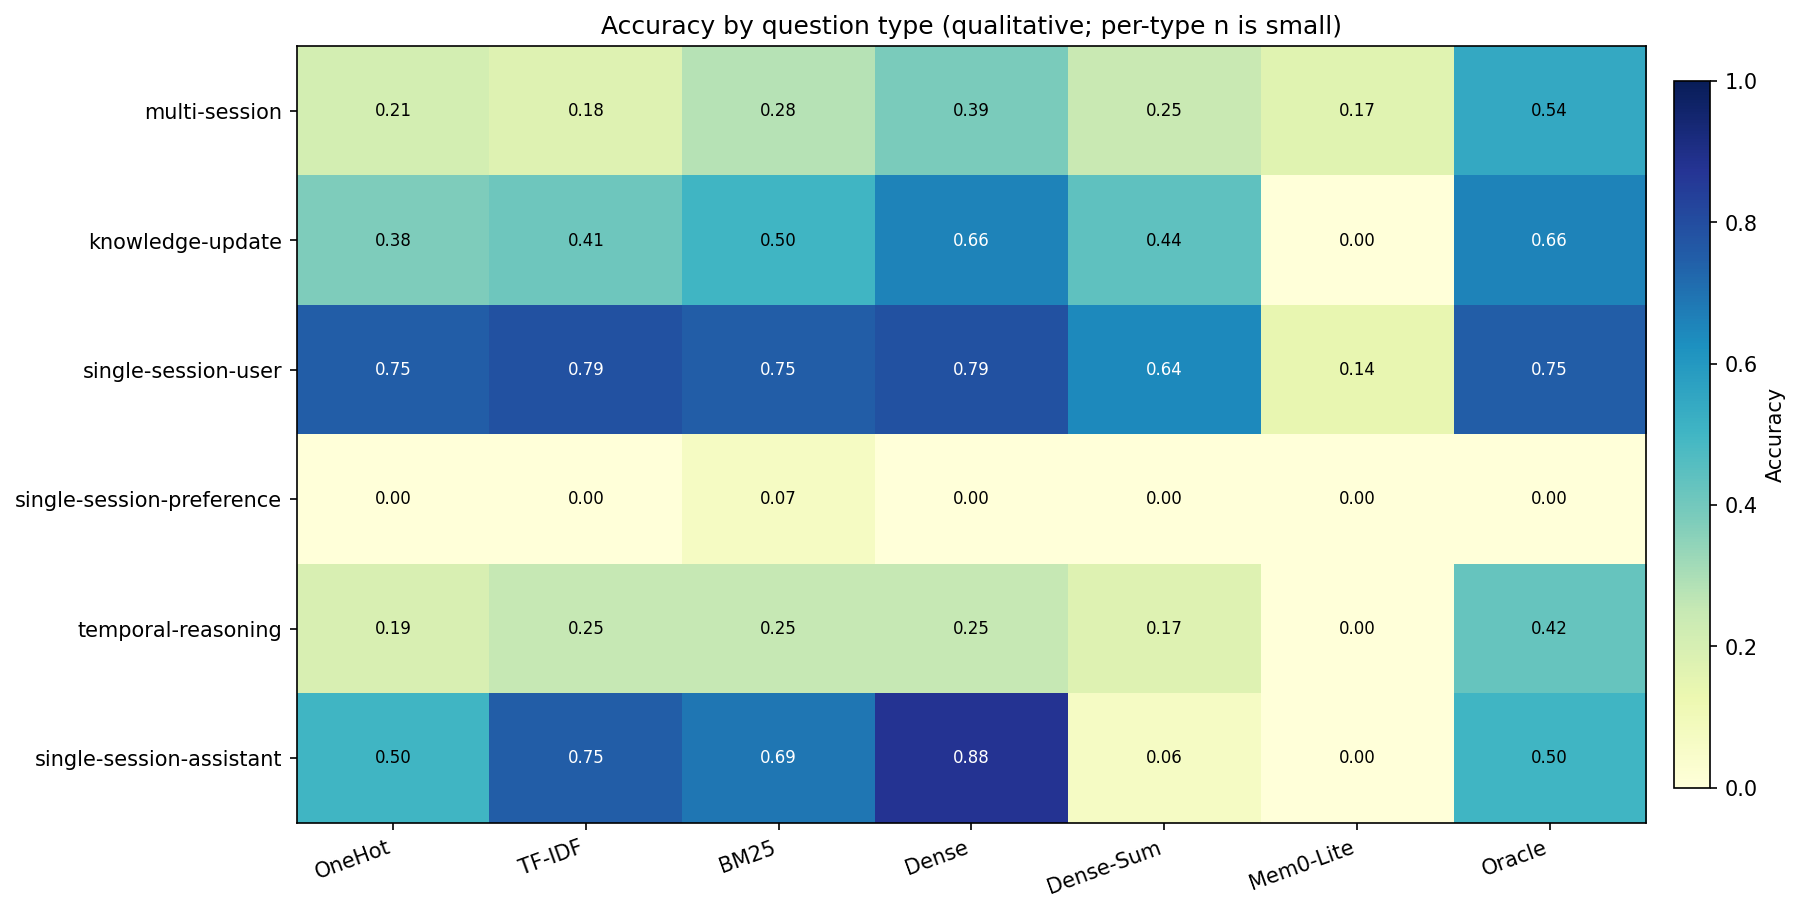
\includegraphics[width=0.92\textwidth]{figs/per_type_heatmap.png}
\caption{Accuracy stratified by LongMemEval-S question type
(qualitative; per-type $n$ is small).}
\label{fig:heat}
\end{figure*}

%================================================
\section{Diagnosis: why does construction hurt?}
\label{sec:diagnosis}

The two regressions above share an unusual property: they go in the
\emph{opposite} direction of the published intuition. Sentence-level
facts are supposed to be cleaner than passage chunks, and an update
agent is supposed to suppress contradictions; instead, both
strategies degrade accuracy. We therefore inspected the actual
retrieved memories on a sample of failed questions to understand
the mechanism.

For Mem0-Lite, the average number of returned memories is 7.06 per
question, with no question hitting the empty-memory case, so the
retriever and the prompt assembly are not the issue. What is
striking is the content. On a question asking ``how much more
expensive was the taxi ride'' (gold: ``\$6''), the top retrieved
memory is ``the user recently returned from a photo shoot with his
sister and her kids.'' On a question asking ``how many sessions of
the bereavement support group did I attend'' (gold: ``five''), the
top memory is a paragraph on misinformation in politics. The
problem is twofold. The 7B extractor, when prompted to produce
typed memory items, frequently produces statements about \emph{the
content of the conversation} rather than about \emph{the user},
including off-topic sentences from chit-chat turns. Worse, the
update agent's add/update/delete decisions are noisy enough that
those off-topic statements survive into the final memory bank. Once
that has happened, no encoder can rescue the retrieval: the literal
``\$6'' is not anywhere in the bank to be retrieved.

For Dense-Summarised, the same mechanism appears in a milder form.
The summariser is asked for at most twelve facts per session, which
imposes a hard upper bound on what survives the construction stage.
Numbers and proper nouns are exactly the tokens that survive
LLM paraphrasing the worst, because they are easily replaced by
generic phrasings (``the user discussed the price of a recent
ride''), and once the literal token is gone the encoder cannot match
it back to the question. The shared cross-encoder reranker cannot
recover information that was discarded in the construction stage.

A single explanation accounts for both regressions:
\textbf{at the 7B-class generator scale we tested, any LLM
construction stage is a lossy text-to-text channel that strips out
the literal numbers, dates and entity strings that the retriever
needs}. The cross-encoder reranker mitigates the noise on the
encoder side but cannot synthesise information that has already
been discarded.

%================================================
\section{Comparison: Pros and Cons}
\label{sec:compare}

To make the trade-offs explicit, Table~\ref{tab:proscons} summarises
the strengths and weaknesses of each retriever as observed in this
study. Two patterns recur. First, accuracy is dominated by whether
the retriever preserves \emph{literal} tokens (numbers, dates,
entity strings) rather than by how cleanly it organises information.
Second, every additional LLM call on the construction side multiplies
both wall-clock latency and cumulative tokens by roughly an order of
magnitude, so the construction stage has to recover at least that
much accuracy to break even, which it does not in our setting.

\begin{table*}[t!]
\centering
\footnotesize
\setlength{\tabcolsep}{6pt}
\renewcommand{\arraystretch}{1.25}
\begin{tabular}{@{}p{2.2cm} p{5.8cm} p{7.5cm}@{}}
\toprule
\textbf{System} & \textbf{Pros} & \textbf{Cons} \\
\midrule
One-hot          & Trivial to implement, no GPU, no hyper-parameters. & Ignores term frequency; weakest accuracy of the seven. \\
TF-IDF           & Captures term salience; CPU-only; very low latency. & Pure lexical match; hurt by paraphrase or synonyms. \\
BM25             & Strong sparse baseline; no GPU; ties TF-IDF here. & Exact-match only; saturates without semantic information. \\
Dense+rerank     & Best accuracy/cost ratio; matches Oracle within CI; off-the-shelf weights. & Needs a sentence encoder and a cross-encoder on GPU; not portable to CPU. \\
Dense-Summarised & Memory items are short and human-readable; useful for inspection. & 20-point accuracy drop vs.\ Dense; one LLM call per session ($\approx$70\,s/q); 100$\times$ more input tokens. \\
Mem0-Lite (7B)   & Richest construction interface (four operations, typed items); closest to the published Mem0 design. & Worst accuracy; two LLM calls per turn ($\approx$252\,s/q); off-topic memories dominate the bank on a 7B extractor. \\
Oracle           & Retrieval-perfect upper bound; isolates the generator-side ceiling at 0.56. & Infeasible in practice (uses gold supporting-turn flags). \\
\bottomrule
\end{tabular}
\caption{Pros and cons of the seven retrievers, summarising the
quantitative results in Table~\ref{tab:results} and the qualitative
diagnosis in \S\ref{sec:diagnosis}.}
\label{tab:proscons}
\end{table*}

%================================================
\section{Discussion and Limitations}
\label{sec:discuss}

\paragraph{What the negative result is, and is not.}
The result is not that ``Mem0 does not work''. The original Mem0
paper reports its gains on top of GPT-4o, with proprietary prompts
and a much larger extractor; it is entirely consistent with our
experiments that the same recipe with a 7B open-weight extractor
underperforms a vanilla Dense + reranker pipeline. What our results
show is that the gap between published numbers and a small-budget
deployment is not a small calibration: the sign of the construction
effect flips. Practitioners who cannot afford a frontier extractor
are, in our setting, better served by spending the budget on a
strong reranker than on an LLM construction stage.

\paragraph{Why Dense matches Oracle.}
A reader might worry that Oracle is simply too easy on this
benchmark. We do not think this reading is correct. Oracle is only
0.56 absolute, which means that 44\% of questions are unanswered by
the generator even when given the gold supporting turns; the
residual error is therefore in the generator, not in retrieval.
Dense also wins eight pairs that Oracle loses, and loses nine that
Oracle wins, so the parity is not the result of identical
predictions. Within the 1024-token budget, Dense + reranker is
finding most of the same supporting evidence that the gold flags
identify.

\paragraph{Threats to validity.}
(1) The judge is a different family from the generator
(DeepSeek vs.\ Qwen), but it is itself an LLM; agreement with a
human grader is not measured here, and a 50-sample human spot-check
would be an obvious refinement. (2) LongMemEval-S is a single
benchmark and English-only;
LOCOMO~\citep{maharana2024locomo} would be the natural next step.
(3) All systems are evaluated at a 1024-token budget; a budget sweep
might re-open a window in which finer-granularity facts pay off,
because the budget itself becomes the bottleneck. (4) Results
should not be extrapolated to a larger extractor: a 70B-class
extractor would plausibly produce cleaner memory items, but
verifying that is out of scope on a single A800. (5) Per-type
accuracies are reported but should not be treated as significance:
the per-type counts are small enough that a single question moves
the rate by 10--20 points.

%================================================
\section{Conclusion}
\label{sec:conclude}

A simple Dense + reranker retriever, run within a fixed
1024-token context budget on a 7B open-weight generator, already
matches the retrieval-perfect Oracle on LongMemEval-S. Adding an
LLM construction stage on top of it (either by summarising sessions
into facts or by running a Mem0-style four-operation update agent)
decreases accuracy, increases latency by one to two orders of
magnitude, and increases cumulative input tokens by roughly the
same factor. The diagnosis is that LLM construction at this scale
is a lossy paraphrasing channel that discards the literal tokens
the retriever needs. Under a small open-weight generator, then, the
budget is better spent on the retriever and the reranker than on
the construction stage. Whether this trade-off flips at frontier
extractor scale, and whether parametric or graph-structured memory
escapes the same channel limitation, are the natural follow-up
questions for our companion survey~\citep{yang2026survey}.

%================================================
\bibliography{custom}

\appendix

\section{Prompts}
\sloppy
The four prompt templates used in the experiments are released
verbatim alongside the code: extraction in
\texttt{prompts/extract.txt}, the four-operation update in
\texttt{prompts/update.txt}, QA generation in
\texttt{prompts/qa.txt}, and LLM-as-judge in
\texttt{prompts/judge.txt}.

\section{Hyper-parameters}
\sloppy
All experiments use seed 42, a top-$k{=}50$ shortlist, a 1024-token
context budget, the BGE-M3 encoder, and
\texttt{bge-reranker-base} as the cross-encoder (applied to both
Dense and Dense-Summarised, top-32 candidates re-ranked). Decoding
is greedy (\texttt{temperature 0}, \texttt{max\_new\_tokens 512}).
The Mem0-Lite extractor and updater both use the same
Qwen2.5-7B-Instruct as the generator, with the JSON-only prompts
under \texttt{prompts/}. The judge uses \texttt{deepseek-v4-flash}
via the OpenAI-compatible API.

\end{document}
